\documentclass[border=4pt]{standalone}
\usepackage[T1]{fontenc}
\usepackage{helvet}
\renewcommand\familydefault{\sfdefault}
\usepackage{tikz}
\usetikzlibrary{positioning,shapes.geometric,arrows.meta,calc,fit}

\begin{document}
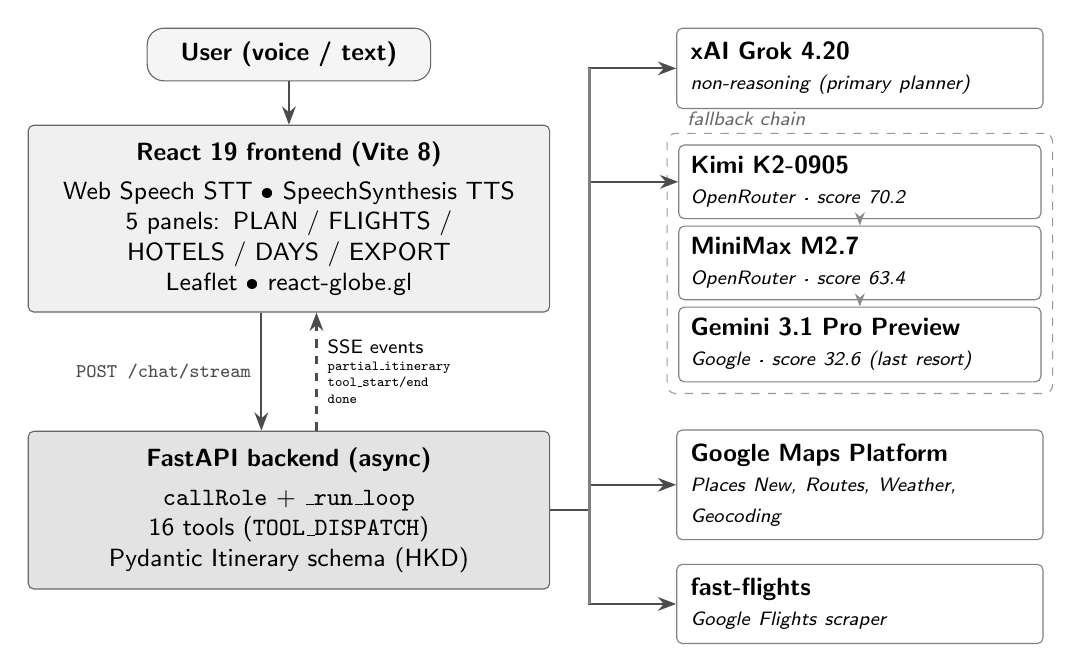
\begin{tikzpicture}[
  font=\small,
  >=Stealth,
  node distance=0.5cm,
  every node/.style={align=center},
  layerbox/.style={draw=black!60, fill=#1, rounded corners=2pt,
                   minimum width=6.6cm, inner sep=6pt, text width=6.2cm},
  extbox/.style={draw=black!50, fill=white, rounded corners=2pt,
                 minimum width=4.6cm, inner sep=5pt, text width=4.3cm, align=left},
  arr/.style={->, thick, black!70},
  retarr/.style={->, thick, black!70, dashed},
]

% --- Left column: user → frontend → backend ---
\node[draw=black!60, fill=gray!8, rounded corners=6pt,
      minimum width=3.6cm, inner sep=5pt]
  (user) {\textbf{User (voice / text)}};

\node[layerbox=gray!12, below=0.55cm of user] (frontend) {%
  \textbf{React 19 frontend (Vite 8)}\\[3pt]
  \small Web Speech STT \textbullet{} SpeechSynthesis TTS\\
  5 panels: PLAN / FLIGHTS / HOTELS / DAYS / EXPORT\\
  Leaflet \textbullet{} react-globe.gl%
};

\node[layerbox=gray!22, below=1.5cm of frontend] (backend) {%
  \textbf{FastAPI backend (async)}\\[3pt]
  \small \texttt{callRole} + \texttt{\_run\_loop}\\
  16 tools (\texttt{TOOL\_DISPATCH})\\
  Pydantic Itinerary schema (HKD)%
};

% --- Right column: LLMs + tools, top-aligned with the User row ---
\node[extbox, anchor=north west]
  (grok) at ([xshift=1.6cm]backend.east |- user.north) {%
  \textbf{xAI Grok 4.20}\\
  \textit{\scriptsize non-reasoning (primary planner)}%
};
\node[extbox, below=0.45cm of grok, minimum width=4.6cm,
      text width=4.3cm, inner sep=4pt] (fb1) {%
  \textbf{Kimi K2-0905}\\
  \textit{\scriptsize OpenRouter \textperiodcentered{} score 70.2}%
};
\node[extbox, below=0.08cm of fb1, minimum width=4.6cm,
      text width=4.3cm, inner sep=4pt] (fb2) {%
  \textbf{MiniMax M2.7}\\
  \textit{\scriptsize OpenRouter \textperiodcentered{} score 63.4}%
};
\node[extbox, below=0.08cm of fb2, minimum width=4.6cm,
      text width=4.3cm, inner sep=4pt] (fb3) {%
  \textbf{Gemini 3.1 Pro Preview}\\
  \textit{\scriptsize Google \textperiodcentered{} score 32.6 (last resort)}%
};
\node[draw=black!40, dashed, rounded corners=3pt, inner sep=4pt,
      fit=(fb1)(fb2)(fb3),
      label={[font=\scriptsize\itshape, text=black!60, anchor=south west,
              xshift=4pt, yshift=-1pt]north west:fallback chain}]
  (fbgroup) {};
\draw[->, black!45, thin] (fb1.south) -- (fb2.north);
\draw[->, black!45, thin] (fb2.south) -- (fb3.north);

\node[extbox, below=0.45cm of fbgroup] (gmaps) {%
  \textbf{Google Maps Platform}\\
  \textit{\scriptsize Places New, Routes, Weather, Geocoding}%
};
\node[extbox, below=0.3cm of gmaps] (ff) {%
  \textbf{fast-flights}\\
  \textit{\scriptsize Google Flights scraper}%
};

% --- Arrows in left column ---
\draw[arr] (user.south) -- (frontend.north);

\draw[arr]
  ([xshift=-0.35cm]frontend.south) --
  node[left, font=\scriptsize, midway]
    {\texttt{POST /chat/stream}}
  ([xshift=-0.35cm]backend.north);
\draw[retarr]
  ([xshift=0.35cm]backend.north) --
  ([xshift=0.35cm]frontend.south);
\node[anchor=west, font=\scriptsize, align=left, inner sep=1pt,
      fill=white, rounded corners=1pt]
  at ($([xshift=0.35cm]backend.north)!0.5!([xshift=0.35cm]frontend.south)
      + (0.10cm,0)$) {%
    SSE events\\[-2pt]
    \texttt{\tiny partial\_itinerary}\\[-2pt]
    \texttt{\tiny tool\_start/end}\\[-2pt]
    \texttt{\tiny done}%
  };

% --- Orthogonal connectors: backend.east → vertical backbone → target.west ---
% Define the backbone x-coordinate (0.5 cm to the right of backend.east)
\coordinate (spine) at ([xshift=0.5cm]backend.east);

% Single arrow exits backend.east, jogs to spine, branches to each target
\draw[arr] (backend.east) -- ++(0.5cm,0) |- (grok.west);
\draw[arr] (backend.east) -- ++(0.5cm,0) |- (fb1.west);
\draw[arr] (backend.east) -- ++(0.5cm,0) |- (gmaps.west);
\draw[arr] (backend.east) -- ++(0.5cm,0) |- (ff.west);

% Vertical spine connects all branch points so the backbone reads as one line
\draw[black!50, thick]
  (spine |- grok.west) -- (spine |- ff.west);

\end{tikzpicture}
\end{document}
